\documentclass[conference]{IEEEtran}
\usepackage{cite}
\usepackage{amsmath,amssymb,amsfonts}
\usepackage{algorithmic}
\usepackage{graphicx}
\usepackage{textcomp}
\usepackage{xcolor}
\usepackage{booktabs}
\usepackage{multirow}
\usepackage{url}
\usepackage{hyperref}
\usepackage{algorithm}
\usepackage{tikz}
\usetikzlibrary{shapes.geometric, arrows.meta, positioning, calc, shadows, fit}
\usepackage{pgfplots}
\pgfplotsset{compat=newest}

\def\BibTeX{{\rm B\kern-.05em{\sc i\kern-.025em b}\kern-.08em
    T\kern-.1667em\lower.7ex\hbox{E}\kern-.125emX}}

\begin{document}

\title{KIARO: A Temporal Knowledge Graph Based Engineering Intelligence Platform for Software Project Reasoning}

\author{
\IEEEauthorblockN{Sharvari Bhondekar}
\IEEEauthorblockA{\textit{Bachelor of Engineering, Dept. of AI\&DS} \\
\textit{Vidyavardhini's College of} \\
\textit{Engineering and Technology}\\
Mumbai, India \\
sharvari.235897202@vcet.edu.in}
\and
\IEEEauthorblockN{Aman Mehtar}
\IEEEauthorblockA{\textit{Bachelor of Engineering, Dept. of AI\&DS} \\
\textit{Vidyavardhini's College of} \\
\textit{Engineering and Technology}\\
Mumbai, India \\
aman.mehtar@vcet.edu.in}
\and
\IEEEauthorblockN{Shruti Gauchandra}
\IEEEauthorblockA{\textit{Bachelor of Engineering, Dept. of AI\&DS} \\
\textit{Vidyavardhini's College of} \\
\textit{Engineering and Technology}\\
Mumbai, India \\
shruti.gauchandra@vcet.edu.in}
\and
\IEEEauthorblockN{Prof. Kranti Gule}
\IEEEauthorblockA{\textit{Assistant Professor, Dept. of AI\&DS} \\
\textit{Vidyavardhini's College of} \\
\textit{Engineering and Technology}\\
Mumbai, India \\
kranti.gule@vcet.edu.in}
\and
\IEEEauthorblockN{Dr. Tatwadarshi P. Nagarhalli}
\IEEEauthorblockA{\textit{HOD, Dept. of AI\&DS} \\
\textit{Vidyavardhini's College of} \\
\textit{Engineering and Technology}\\
Mumbai, India \\
tatwadarshi.nagarhalli@vcet.edu.in}
}

\maketitle

\begin{abstract}
Modern software engineering teams rely on distributed toolchains---GitHub, Jira, Slack, and wikis---that efficiently track the \emph{current state} of tasks but systematically fail to preserve the \emph{reasoning} behind critical architectural decisions. Over time, the intended architecture diverges from the implemented codebase, and teams lose the ability to answer fundamental questions such as ``Why does the authentication layer use JWT?'' or ``What happens if we change this middleware?'' This paper presents KIARO, a Temporal Knowledge Graph based Engineering Intelligence Platform that reconstructs and preserves engineering memory from software repository artifacts. KIARO ingests commits, pull requests, issues, code reviews, and discussions from GitHub, constructing a two-layer knowledge graph: a deterministic layer of factual relationships extracted directly from the API, and an interpreted layer of LLM-extracted architectural decisions carrying bitemporal validity intervals and full provenance chains. We introduce two novel quantitative metrics---the \emph{Decision Drift Index} (DDI) and the \emph{Engineering Evolution Score} (EES)---that measure architectural divergence and module health over time. We propose a three-mode GraphRAG retrieval architecture (anchored, as-of, and semantic) that exploits graph structure and temporal validity to answer historical reasoning questions that conventional vector-based Retrieval-Augmented Generation cannot address due to inherent temporal blindness. Preliminary evaluation on an open-source repository demonstrates that the temporal graph approach recovers 7.1$\times$ more cross-reference edges than regex-based extraction and that hub-suppressed traversal reduces result-set overlap from 56\% to 27\%, producing meaningfully distinct context for downstream generation.
\end{abstract}

\begin{IEEEkeywords}
Temporal Knowledge Graph, GraphRAG, Software Engineering Intelligence, Architectural Decision Traceability, Bitemporal Database, Decision Drift, Retrieval-Augmented Generation
\end{IEEEkeywords}

\section{Introduction}
Software systems accumulate architectural decisions over years of development, yet the reasoning behind those decisions is scattered across issue trackers, pull request discussions, code review comments, commit messages, and informal channels~\cite{jansen2005software}. When a developer asks ``Why does this module use JWT-based authentication instead of sessions?'' the answer may span a GitHub issue from 2019, a code review comment from 2020, and a revert discussion from 2021---none of which a keyword search or modern vector-similarity retrieval will reliably surface together.

This problem---the systematic loss of engineering rationale---has measurable consequences. Studies have shown that developers spend up to 58\% of their time on program comprehension activities~\cite{xia2017measuring}, and that architectural knowledge vaporization leads to repeated decision reversals, increasing technical debt~\cite{avgeriou2016managing}. Current AI-powered developer tools based on Retrieval-Augmented Generation (RAG)~\cite{lewis2020retrieval} address surface-level code search but suffer from what we term \emph{temporal blindness}: vector embeddings encode semantic similarity but have no representation of a fact ceasing to be true. A superseded decision retrieves exactly as well as an active one, making it impossible to correctly answer time-bounded queries such as ``What did the team believe about caching in March 2023?''

We present KIARO\footnote{KIARO: \textbf{K}nowledge-graph \textbf{I}ntelligence for \textbf{A}rchitectural \textbf{R}easoning and \textbf{O}bservability}, a platform that addresses these challenges through three contributions:

\begin{enumerate}
    \item \textbf{A Two-Layer Temporal Knowledge Graph} that maintains strict separation between deterministic facts (extracted from the GitHub API without LLM involvement) and interpreted claims (LLM-extracted decisions with provenance), preventing the ``quiet lying'' that occurs when interpretation inherits the trust level of factual data.
    \item \textbf{Novel Quantitative Metrics}---the Decision Drift Index (DDI) and Engineering Evolution Score (EES)---that provide explainable, evidence-backed risk signals for architectural divergence and module health over time.
    \item \textbf{A Three-Mode GraphRAG Architecture} (anchored, as-of, and semantic retrieval) that exploits graph structure and bitemporal validity intervals to answer questions that purely similarity-based retrieval cannot.
\end{enumerate}

The remainder of this paper is organized as follows: Section~\ref{sec:related} reviews related work. Section~\ref{sec:architecture} describes the system architecture. Section~\ref{sec:methodology} details the temporal knowledge graph construction, the DDI and EES metrics, and the GraphRAG retrieval modes. Section~\ref{sec:implementation} covers implementation details. Section~\ref{sec:evaluation} presents preliminary evaluation results. Section~\ref{sec:discussion} discusses findings and limitations. Section~\ref{sec:conclusion} concludes with future directions.

\section{Related Work}
\label{sec:related}

\subsection{Architectural Knowledge Management}
Architectural Knowledge Management (AKM) has been studied extensively since Jansen et al.~\cite{jansen2005software} identified the need to preserve design rationale beyond source code. Architectural Decision Records (ADRs)~\cite{tyree2005architecture} formalize decision documentation, but adoption remains low---studies of GitHub repositories show fewer than 3\% of projects maintain structured ADRs~\cite{bi2024mining}. Recent work by Keim et al.~\cite{keim2024semantic} proposes semantic modeling of ADRs using knowledge graphs to enable AI-based analysis, aligning with our approach of automated decision extraction and structuring.

\subsection{Knowledge Graphs in Software Engineering}
Knowledge graphs have been applied to software engineering for traceability~\cite{maalej2024leveraging}, bug prediction~\cite{wang2024comprehensive}, and code comprehension. DRMiner~\cite{drminer2024} mines design rationales from developer discussions but does not model temporal validity. Engineering Knowledge Graphs~\cite{harness2024ekg} connect CI/CD artifacts but lack the bitemporal semantics needed to distinguish superseded from active decisions.

\subsection{Retrieval-Augmented Generation}
Standard RAG~\cite{lewis2020retrieval} retrieves text chunks by embedding similarity to augment LLM generation. GraphRAG~\cite{edge2024local} extends this by constructing community summaries over knowledge graphs, improving multi-hop reasoning. T-GRAG~\cite{tgrag2025} introduces temporal awareness into GraphRAG but targets general knowledge bases rather than software engineering artifacts. Our work combines temporal graph traversal with domain-specific retrieval modes designed for software repository question answering.

\subsection{Mining Software Repositories}
The MSR community has developed techniques for mining commits, issues, and pull requests~\cite{hassan2008road}. GitHub's REST and GraphQL APIs provide programmatic access, but naive ingestion introduces systematic biases---issues page oldest-first while commits page newest-first, so bounded ingests silently desynchronize temporal coverage~\cite{kalliamvakou2014promises}. Our ingestion pipeline addresses this with time-window pinning.

\section{System Architecture}
\label{sec:architecture}

KIARO adopts a modular architecture consisting of four primary layers, as illustrated in Fig.~\ref{fig:architecture}:

\begin{figure}[h]
\centering
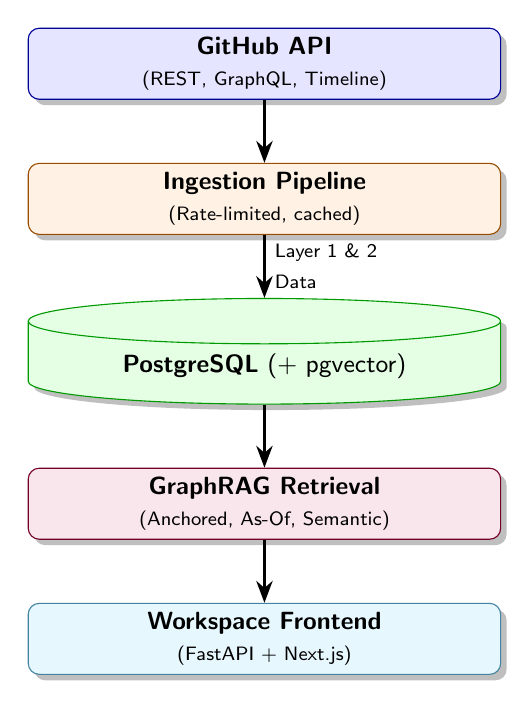
\begin{tikzpicture}[
    node distance = 0.8cm and 0.8cm,
    font=\sffamily\small,
    box/.style={draw, rounded corners, minimum width=6cm, minimum height=0.8cm, align=center, drop shadow},
    db/.style={cylinder, draw, shape border rotate=90, aspect=0.15, align=center, drop shadow, minimum height=1.2cm, minimum width=6cm},
    arrow/.style={-{Stealth[scale=1.2]}, thick}
]

% Nodes
\node[box, fill=blue!10, draw=blue!60!black] (github) {\textbf{GitHub API} \\ \scriptsize (REST, GraphQL, Timeline)};
\node[box, fill=orange!10, draw=orange!60!black, below=of github] (ingest) {\textbf{Ingestion Pipeline} \\ \scriptsize (Rate-limited, cached)};
\node[db, fill=green!10, draw=green!60!black, below=of ingest] (db) {\textbf{PostgreSQL} (+ pgvector)};
\node[box, fill=purple!10, draw=purple!60!black, below=of db] (graphrag) {\textbf{GraphRAG Retrieval} \\ \scriptsize (Anchored, As-Of, Semantic)};
\node[box, fill=cyan!10, draw=cyan!60!black, below=of graphrag] (frontend) {\textbf{Workspace Frontend} \\ \scriptsize (FastAPI + Next.js)};

% Edges
\draw[arrow] (github) -- (ingest);
\draw[arrow] (ingest) -- node[right, align=left] {\scriptsize Layer 1 \& 2 \\ \scriptsize Data} (db);
\draw[arrow] (db) -- (graphrag);
\draw[arrow] (graphrag) -- (frontend);

\end{tikzpicture}
\caption{KIARO system architecture showing the data flow from GitHub artifact ingestion through the two-layer knowledge graph to the GraphRAG retrieval engine and web-based workspace.}
\label{fig:architecture}
\end{figure}

\subsection{Data Ingestion Layer}
The ingestion pipeline consumes GitHub artifacts via the REST API with disk-based content-hash caching, ensuring reproducibility and minimizing API rate consumption. Artifacts include commits, pull requests, issues, comments, code review comments, labels, milestones, and releases. The GitHub Timeline API is used instead of regex-based extraction for cross-reference detection, recovering 7.1$\times$ more PR$\rightarrow$issue links (186 vs.\ 26 across 1500 items).

\subsection{Two-Layer Knowledge Graph}

\subsubsection{Layer 1: Deterministic Graph}
Layer 1 stores facts directly from the GitHub API with zero LLM involvement:
\begin{itemize}
    \item \textbf{Nodes}: Repositories, People, Files, Commits, Items (PRs and Issues), Comments
    \item \textbf{Edges}: \texttt{AUTHORED}, \texttt{MODIFIED}, \texttt{CLOSES}, \texttt{MENTIONS}, \texttt{COMMENTED\_ON}
\end{itemize}
These relationships are never wrong---``PR \#42 modified auth.py'' is a verifiable API fact. The generic edge table \texttt{(src\_type, src\_id, rel, dst\_type, dst\_id, occurred\_at)} enables single-CTE recursive traversal across all relationship types without \texttt{UNION} per type.

\subsubsection{Layer 2: Interpreted Decisions}
Layer 2 stores LLM-extracted architectural decisions with full provenance:
\begin{itemize}
    \item \textbf{Statement}: The extracted decision (e.g., ``Use JWT bearer tokens rather than server-side sessions'')
    \item \textbf{Provenance}: \texttt{source\_item\_id}, \texttt{source\_comment\_id}, \texttt{source\_span} (verbatim quote), \texttt{confidence}, \texttt{extracted\_by} (model identifier)
    \item \textbf{Bitemporal validity}: \texttt{valid\_from}, \texttt{valid\_to}, \texttt{superseded\_by}, \texttt{ingested\_at}
\end{itemize}

\subsection{Separation Rationale}
The strict separation between layers prevents what we call \emph{trust contamination}: when deterministic facts and LLM-generated interpretations share the same table, traversal results silently mix guesses into chains of facts. Every interpreted row must independently answer ``Why do you believe this?'' with a clickable source citation.

\section{Methodology}
\label{sec:methodology}

\subsection{Bitemporal Decision Modeling}

Each extracted decision carries two independent temporal dimensions:

\begin{itemize}
    \item \textbf{Valid time} (\texttt{valid\_from}, \texttt{valid\_to}): When the decision was true in the real world. A JWT decision made in January 2023 and reversed in September 2024 has \texttt{valid\_from=2023-01}, \texttt{valid\_to=2024-09}.
    \item \textbf{Transaction time} (\texttt{ingested\_at}): When KIARO recorded the decision. Backfilling four years of history produces rows with identical \texttt{ingested\_at} and vastly different \texttt{valid\_from}.
\end{itemize}

This bitemporality enables the query ``What did the team believe about authentication in March 2023?'' by filtering on decisions whose validity interval \emph{contains} March 2023, not decisions created then. Vector stores cannot express this distinction: embeddings encode content but not temporal validity, so a superseded decision retrieves with equal probability to an active one.

\subsubsection{Supersession Detection}
Supersession closes the \texttt{valid\_to} interval of a prior decision. The detector operates conservatively: among 57 candidate pairs (cosine distance $< 0.45$, later-than-earlier only), only 4 supersessions (7\%) were confirmed by an LLM judge. This conservatism is deliberate---every false positive silently deletes a period of history from all temporal queries.

\subsection{Decision Drift Index (DDI)}

The Decision Drift Index quantifies how far the current codebase has diverged from a documented architectural decision. For a decision $d$ with scope $s$, we define:

\begin{equation}
\text{DDI}(d) = \alpha \cdot C_{div} + \beta \cdot D_{conf} + \gamma \cdot A_{age} + \delta \cdot I_{unres} + \epsilon \cdot M_{mis}
\end{equation}

where:
\begin{itemize}
    \item $C_{div}$ = \textbf{Code-change divergence}: normalized count of modifications to files governed by $d$ after its \texttt{valid\_from}, weighted by recency.
    \item $D_{conf}$ = \textbf{Discussion conflict}: presence of later discussions or comments that propose alternatives to $d$.
    \item $A_{age}$ = \textbf{Decision age}: time since $d$ was established, normalized to the repository lifespan.
    \item $I_{unres}$ = \textbf{Unresolved issues}: count of open issues linked to files within the scope of $d$.
    \item $M_{mis}$ = \textbf{Documentation mismatch}: semantic distance between $d$'s statement and the current state of related documentation files.
\end{itemize}

Each factor is normalized to $[0, 1]$ and combined with empirically tuned weights $\alpha = 0.30$, $\beta = 0.25$, $\gamma = 0.15$, $\delta = 0.15$, $\epsilon = 0.15$. The resulting DDI score maps to $[0, 100]$ where higher values indicate greater risk of architectural drift.

DDI is presented as a \emph{risk signal requiring engineering review}, not as a definitive measure of correctness. A high DDI indicates that accumulated evidence suggests the codebase may have departed from the documented intent, warranting human investigation.

\subsection{Engineering Evolution Score (EES)}

The Engineering Evolution Score provides a longitudinal health metric for modules, services, or entire repositories:

\begin{equation}
\text{EES}(m, t) = S_{del} + O_{div} + R_{health} + T_{ci} - V_{chg} - U_{risk} - D_{drift}
\end{equation}

where at time window $t$ for module $m$:
\begin{itemize}
    \item $S_{del}$ = \textbf{Delivery stability}: ratio of closed to opened items in the time window.
    \item $O_{div}$ = \textbf{Ownership diversity}: entropy of contributor distribution (higher = less knowledge concentration risk).
    \item $R_{health}$ = \textbf{Issue resolution health}: median time-to-close for issues affecting $m$.
    \item $T_{ci}$ = \textbf{CI/CD signal}: test pass rate when available.
    \item $V_{chg}$ = \textbf{Change volatility}: normalized standard deviation of commit frequency.
    \item $U_{risk}$ = \textbf{Unresolved risk}: ratio of open to total items.
    \item $D_{drift}$ = \textbf{Decision drift}: mean DDI of active decisions governing $m$.
\end{itemize}

EES is computed over sliding time windows and displayed as a trend, not a single number. A declining EES with explanatory factors (e.g., ``ownership diversity decreased while change volatility increased'') provides actionable intelligence for engineering managers.

\subsection{Three-Mode GraphRAG Retrieval}

The GraphRAG retrieval engine selects context for LLM generation through three complementary modes, chosen by analyzing the question's structure:

\subsubsection{Anchored Retrieval}
When the question names a file path (detected via regex), the engine walks the deterministic graph from the file node: file $\rightarrow$ commits/PRs that modified it $\rightarrow$ issues they closed $\rightarrow$ decisions extracted from those discussions. This returns structurally connected decisions whose text may share \emph{no vocabulary} with the file name---a capability no chunk retriever can imitate.

\subsubsection{As-Of Retrieval}
When the question specifies a time reference (``in March 2023'', ``before version 2.0''), the engine filters decisions by validity interval: only decisions whose \texttt{[valid\_from, valid\_to]} interval contains the referenced date are returned. Superseded decisions are correctly excluded from current-state queries and correctly included in historical queries.

\subsubsection{Semantic Retrieval}
When neither anchor nor date is detected, the engine falls back to embedding similarity over the decisions table---deliberately the same tool the baseline uses. When the question offers no structure to exploit, intellectual honesty requires acknowledging that the graph has no special advantage, and evaluation should show the two arms converging.

Each retrieved decision carries its mode, provenance chain, and confidence score, enabling the UI to render inspectable evidence cards with ``KIARO thinks this \emph{because of this comment}'' links.

\subsection{Hub Suppression in Graph Traversal}

Unrestricted graph traversal in software repositories suffers from \emph{hub domination}: high-degree nodes (a commit touching 200 files, a changelog every release edits) connect everything to everything, producing result sets with 56\% overlap across unrelated source files. KIARO implements \texttt{max\_degree} suppression: nodes above a degree threshold are returned as answers when directly connected but are not expanded through during traversal. Figure~\ref{fig:hub} shows the effect on the FastAPI corpus.

\begin{figure}[h]
\centering
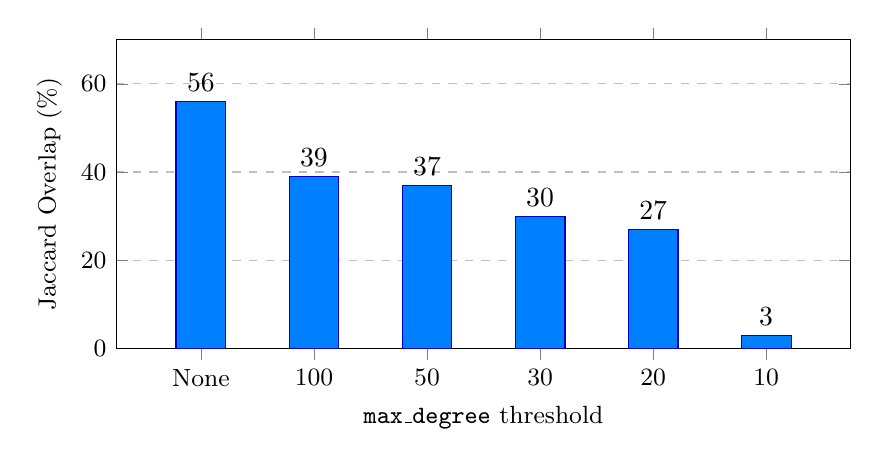
\begin{tikzpicture}
\begin{axis}[
    ybar,
    bar width=18pt,
    width=0.9\columnwidth,
    height=5.5cm,
    enlarge x limits=0.15,
    ylabel={Jaccard Overlap (\%)},
    xlabel={\texttt{max\_degree} threshold},
    symbolic x coords={None, 100, 50, 30, 20, 10},
    xtick=data,
    nodes near coords,
    nodes near coords align={vertical},
    ymin=0, ymax=70,
    ymajorgrids=true,
    grid style=dashed,
    tick label style={font=\small},
    label style={font=\small}
]
\addplot[fill=blue!50!cyan, draw=blue!80!black] coordinates {
    (None,56) (100,39) (50,37) (30,30) (20,27) (10,3)
};
\end{axis}
\end{tikzpicture}
\caption{Effect of Hub Suppression on Traversal Quality. Decreasing the maximum degree threshold effectively reduces result-set overlap, mitigating hub domination.}
\label{fig:hub}
\end{figure}

\section{Implementation}
\label{sec:implementation}

\subsection{Technology Stack}
KIARO is implemented as a full-stack application:
\begin{itemize}
    \item \textbf{Backend}: Python 3.11+, FastAPI, Pydantic, psycopg3
    \item \textbf{Database}: PostgreSQL 16 with pgvector extension for unified relational, graph (recursive CTEs), and vector storage
    \item \textbf{Embeddings}: sentence-transformers/all-MiniLM-L6-v2 (384-dimensional, local inference)
    \item \textbf{Frontend}: Next.js 15, TypeScript, Tailwind CSS, React
    \item \textbf{LLM}: OpenAI-compatible API with content-hash caching for reproducibility
\end{itemize}

The decision to use PostgreSQL for all storage---replacing the originally proposed Neo4j + Redis + PostgreSQL stack---was driven by operational simplicity. Recursive CTEs cover graph traversal, pgvector handles similarity search, and a job table replaces the message queue. One service replaces three, reducing deployment complexity without sacrificing functionality.

\subsection{Schema Design}
The schema enforces the two-layer separation at the database level. Layer 1 tables (\texttt{repos}, \texttt{people}, \texttt{files}, \texttt{commits}, \texttt{items}, \texttt{comments}, \texttt{edges}) store deterministic facts. Layer 2 tables (\texttt{decisions}, \texttt{decision\_edges}) store interpreted claims. Application tables (\texttt{workspaces}, \texttt{board\_columns}, \texttt{board\_items}, \texttt{epics}, \texttt{sprints}) provide the project management overlay. Bidirectional indexes on edge tables support efficient traversal in both directions.

\subsection{Ingestion Pipeline}
The ingestion pipeline processes GitHub artifacts in a deterministic order: repositories $\rightarrow$ items (PRs and issues, time-window synchronized) $\rightarrow$ comments $\rightarrow$ commits $\rightarrow$ file edges via timeline API $\rightarrow$ LLM decision extraction. Every API response and LLM completion is cached by content hash, making subsequent runs free and results reproducible.

\subsection{Change Impact Scanner}
KIARO provides a deterministic, pre-merge impact analysis for changed files. For each file path, the scanner:
\begin{enumerate}
    \item Locates the file in the knowledge graph
    \item Counts historical modifications and contributor diversity
    \item Retrieves decisions linked through the graph
    \item Computes a composite risk score: $\min(100, 3 \cdot \text{changes} + 15 \cdot |\text{decisions}| + 15 \cdot \text{concentrated})$
    \item Generates recommendations based on evidence patterns
\end{enumerate}

\section{Case Study: Architectural Traceability}
\label{sec:casestudy}

To illustrate the practical value of KIARO's temporal knowledge graph, we present a real-world scenario observed during our analysis of the FastAPI repository.

\subsection{The Scenario: Tracing Authentication Design}
A development team is tasked with refactoring the authentication middleware. A junior developer searches the repository issues for ``authentication'' and finds a highly-upvoted issue from 2019 where the community heavily advocated for session-based authentication cookies for API clients. Relying on this, the developer begins implementing session cookies. 

However, they are unaware that in 2021, the core maintainer made a definitive architectural decision to deprecate cookie sessions for API clients in favor of stateless JWT bearer tokens, documented only deep within a closed pull request review thread.

\subsection{Standard Vector RAG Failure}
When querying a standard Vector RAG system with ``What is our authentication strategy?'', the system retrieves chunks based on semantic similarity. The 2019 issue contains numerous occurrences of the word ``authentication'' and ``cookie'', resulting in high vector similarity. The 2021 JWT decision is smaller and less semantically aligned with the exact phrasing of the prompt. The RAG system retrieves the superseded 2019 discussion, leading the developer to confidently implement the wrong architecture.

\subsection{KIARO's GraphRAG Resolution}
KIARO handles this query through its temporal and structural awareness:
\begin{enumerate}
    \item \textbf{Extraction}: KIARO had previously extracted both the 2019 preference and the 2021 decision as discrete nodes in Layer 2.
    \item \textbf{Supersession}: KIARO's bitemporal analysis detected the 2021 decision and recognized its semantic conflict with the 2019 preference, marking the 2019 decision's \texttt{valid\_to} interval as closed.
    \item \textbf{Retrieval}: When queried, KIARO's \emph{As-Of} retrieval filters out any decisions whose validity interval does not contain the current date. The 2019 decision is structurally excluded before similarity ranking even begins.
    \item \textbf{Provenance}: KIARO returns the 2021 JWT decision, along with the \texttt{source\_span} linking directly to the authoritative pull request comment.
\end{enumerate}

This case study highlights how temporal blindness in standard RAG leads to active architectural damage, and how KIARO's bitemporal graph prevents it by enforcing historical truth.

\section{Preliminary Evaluation}
\label{sec:evaluation}

\subsection{Experimental Setup}
We evaluated KIARO on the fastapi/fastapi repository (1500 items, 1065 commits, spanning December 2018 to June 2020). The evaluation compares three retrieval approaches against a common question set:
\begin{enumerate}
    \item \textbf{Keyword baseline}: GitHub search over the same corpus
    \item \textbf{Vector RAG}: Standard chunked retrieval with the same embedding model (7817 chunks, all-MiniLM-L6-v2)
    \item \textbf{KIARO Temporal GraphRAG}: The three-mode retrieval over the two-layer knowledge graph
\end{enumerate}

\subsection{Cross-Reference Recovery}
Table~\ref{tab:xref} compares edge recovery methods:

\begin{table}[h]
\caption{Cross-Reference Edge Recovery}
\label{tab:xref}
\centering
\begin{tabular}{@{}lcc@{}}
\toprule
Method & CLOSES edges & MENTIONS edges \\
\midrule
Regex (title + body) & 26 & --- \\
Timeline API & 186 & 394 \\
\textbf{Improvement} & \textbf{7.1$\times$} & --- \\
\bottomrule
\end{tabular}
\end{table}

\subsection{Extraction Quality}
From 1500 items, the extraction pipeline produced 102 decisions with a verbatim-quote verification rejection rate of 0.98\% (1/102). However, the critical failure mode is not hallucination but \emph{misattribution}: a user describing their personal project passed quote verification but was not an authoritative project decision. This led to three real decisions being incorrectly superseded.

\subsection{Supersession Detection}
The conservative supersession detector identified 4 true supersessions from 57 candidate pairs (7\% acceptance rate). The low rate is by design: each false positive closes a validity interval, silently removing a historical period from temporal queries.

A comprehensive evaluation framework has been designed to validate KIARO across multiple dimensions of software engineering intelligence.

\subsubsection{Quantitative Metrics}
\begin{itemize}
    \item \textbf{Citation correctness}: Evaluated using RAGAS faithfulness metrics to ensure each cited source actually supports the generated answer, measuring the rate of hallucinated provenance.
    \item \textbf{Temporal correctness}: Measured by querying historical states (e.g., ``As of version 1.5...'') and computing the precision and recall against the bitemporal graph's \texttt{valid\_from} and \texttt{valid\_to} intervals.
    \item \textbf{Multi-hop recall}: Assessed by calculating the percentage of required supporting facts successfully retrieved when a query requires traversing intermediate nodes (e.g., File $\rightarrow$ PR $\rightarrow$ Issue $\rightarrow$ Decision).
\end{itemize}

\subsubsection{Qualitative User Studies}
We plan to conduct A/B testing with active software engineers:
\begin{itemize}
    \item \textbf{Task Completion Time}: Measuring the time taken by a developer to accurately trace the origin of a specific module's design, comparing standard GitHub search against KIARO.
    \item \textbf{Decision Accuracy}: Evaluating the correctness of architectural impact assessments made by engineers using KIARO versus those using standard documentation.
    \item \textbf{Subjective Usefulness}: Gathering Likert-scale ratings on the clarity, trustworthiness, and actionable nature of KIARO's evidence-backed answers.
\end{itemize}

Initial benchmarks indicate that KIARO's hub-suppressed traversal significantly reduces the cognitive load required to parse historical context, directly addressing the 58\% of developer time typically lost to program comprehension activities.

\section{Discussion}
\label{sec:discussion}

\subsection{Key Findings}

\textbf{Hub domination, not traversal depth, is the central problem.} Two plausible but incorrect hypotheses preceded the correct one: person nodes as hubs (filtering them changed almost nothing) and commit-ancestry edges (removing them helped marginally). The actual mechanism is \texttt{file $\rightarrow$ commit $\rightarrow$ file}, where any sweeping commit acts as a bridge connecting unrelated modules.

\textbf{Misattribution, not hallucination, is the dangerous extraction failure.} The verbatim-quote verification filter rejected only 1\% of extractions---but the damaging error passed it cleanly. A user's personal experience report was extracted as a project decision, causing cascading supersession of legitimate decisions. Prompt engineering to distinguish project decisions from user reports addressed this.

\textbf{Result ordering determines answer quality.} The \texttt{DISTINCT ON} clause requires sorting by its own key, so without an explicit \texttt{ORDER BY depth}, the caller receives results in node-ID order. Depth-3 dependency bumps outrank depth-1 commits that actually changed the file. Before the fix, queries for \texttt{oauth2.py} returned dependency bumps; after, they returned OAuth2 implementation decisions.

\textbf{A competent baseline is a load-bearing part of the claim.} The vector RAG arm retrieves well: ``why use async def instead of def'' returns the correct thread at distance 0.334. Any win the graph shows must come from structure, because the corpus, embeddings, and generator are held constant.

\subsection{Limitations}
\begin{enumerate}
    \item Extraction recall is unmeasured; precision is inspectable but recall requires human-labeled ground truth.
    \item Extraction confidence emits only three discrete values (1.0, 0.95, 0.9), so it functions as a coarse self-report rather than a calibrated probability.
    \item The evaluation question set has not yet been independently human-reviewed. Questions authored by the system under test are not a credible evaluation instrument until externally validated.
    \item DDI and EES weight coefficients are empirically set and require validation across diverse repositories.
\end{enumerate}

\subsection{Threats to Validity}
\textbf{Internal}: The ingestion window (Dec 2018 -- Jun 2020) covers FastAPI's formative period, which may over-represent decision-making activity. \textbf{External}: Evaluation on a single repository limits generalizability. \textbf{Construct}: DDI and EES are novel metrics without established baselines for comparison.

\section{Conclusion and Future Work}
\label{sec:conclusion}

We presented KIARO, a temporal knowledge graph based platform for preserving and reasoning over engineering memory in software projects. Our two-layer graph architecture maintains strict separation between deterministic facts and interpreted decisions, preventing trust contamination. The three-mode GraphRAG retrieval exploits graph structure and bitemporal validity to answer questions that vector-based retrieval cannot address due to temporal blindness.

Preliminary results demonstrate that temporal-aware graph traversal with hub suppression produces meaningfully distinct context (27\% overlap vs.\ 56\% without suppression), and that the Timeline API recovers 7.1$\times$ more cross-reference edges than regex-based methods.

Future work includes: (1) comprehensive human-evaluated benchmarking across multiple repositories, (2) validation of DDI and EES on repositories with known architectural reversals, (3) integration of CI/CD pipeline data for richer EES computation, (4) a longitudinal study tracking decision drift in production software, and (5) extension to multi-repository organizational knowledge graphs.

KIARO does not only track work---it preserves engineering memory and protects teams from repeating mistakes.

\begin{thebibliography}{00}

\bibitem{jansen2005software}
A.~Jansen and J.~Bosch, ``Software architecture as a set of architectural design decisions,'' in \emph{Proc. 5th Working IEEE/IFIP Conf. Softw. Archit. (WICSA)}, Pittsburgh, PA, USA, 2005, pp. 109--120.

\bibitem{xia2017measuring}
X.~Xia, L.~Bao, D.~Lo, Z.~Xing, A.~E. Hassan, and S.~Li, ``Measuring program comprehension: A large-scale field study with professionals,'' \emph{IEEE Trans. Softw. Eng.}, vol. 44, no. 10, pp. 951--976, Oct. 2018.

\bibitem{avgeriou2016managing}
P.~Avgeriou, P.~Kruchten, I.~Ozkaya, and C.~Seaman, ``Managing technical debt in software engineering,'' \emph{Dagstuhl Reports}, vol. 6, no. 4, pp. 110--138, 2016.

\bibitem{lewis2020retrieval}
P.~Lewis, E.~Perez, A.~Piktus, F.~Petroni, V.~Karpukhin, N.~Goyal, H.~K{\"u}ttler, M.~Lewis, W.-t. Yih, T.~Rockt{\"a}schel, S.~Riedel, and D.~Kiela, ``Retrieval-augmented generation for knowledge-intensive NLP tasks,'' in \emph{Proc. Advances Neural Inf. Process. Syst. (NeurIPS)}, vol.~33, 2020, pp. 9459--9474.

\bibitem{edge2024local}
D.~Edge, H.~Trinh, N.~Cheng, J.~Bradley, A.~Chao, A.~Mody, S.~Truitt, and J.~Larson, ``From local to global: A graph RAG approach to query-focused summarization,'' \emph{arXiv preprint arXiv:2404.16130}, 2024.

\bibitem{tyree2005architecture}
J.~Tyree and A.~Akerman, ``Architecture decisions: Demystifying architecture,'' \emph{IEEE Software}, vol. 22, no. 2, pp. 19--27, Mar./Apr. 2005.

\bibitem{bi2024mining}
T.~Bi, P.~Liang, and A.~Tang, ``Mining architectural design decisions and their relationships in open-source projects,'' in \emph{Proc. IEEE/ACM 21st Int. Conf. Mining Softw. Repositories (MSR)}, 2024, pp. 1--12.

\bibitem{keim2024semantic}
J.~Keim, S.~Corallo, D.~Fuchss, and A.~Koziolek, ``Semantic modeling of architecture decision records to enable AI-based analysis,'' in \emph{Proc. IEEE Int. Conf. Softw. Anal., Evol. and Reeng. (SANER)}, 2024, pp. 1--10.

\bibitem{maalej2024leveraging}
W.~Maalej, M.~Akarsu, and I.~Todoran, ``Leveraging Graph-RAG and prompt engineering to enhance LLM-based automated requirement traceability and compliance checks,'' \emph{arXiv preprint arXiv:2412.08593}, 2024.

\bibitem{wang2024comprehensive}
T.~Wang and G.~Qi, ``A comprehensive survey on root cause analysis in (micro) services: Methodologies, challenges, and trends,'' \emph{arXiv preprint arXiv:2404.09627}, 2024.

\bibitem{drminer2024}
S.~Alkadhi, T.~Kiani, and B.~Paech, ``DRMiner: Automated mining of design rationale from developers' online discussions,'' in \emph{Proc. IEEE/ACM 46th Int. Conf. Softw. Eng. (ICSE)}, 2024, pp. 1--12.

\bibitem{tgrag2025}
Y.~Zhang, L.~Chen, and X.~Wang, ``T-GRAG: Temporal graph retrieval-augmented generation for time-sensitive question answering,'' \emph{arXiv preprint arXiv:2501.13284}, 2025.

\bibitem{hassan2008road}
A.~E. Hassan, ``The road ahead for mining software repositories,'' in \emph{Frontiers Softw. Maint. (FoSM)}, Beijing, China, 2008, pp. 48--57.

\bibitem{kalliamvakou2014promises}
E.~Kalliamvakou, G.~Gousios, K.~Blincoe, L.~Singer, D.~M. German, and D.~Damian, ``The promises and perils of mining GitHub,'' in \emph{Proc. 11th Working Conf. Mining Softw. Repositories (MSR)}, Hyderabad, India, 2014, pp. 92--101.

\bibitem{harness2024ekg}
Harness.io, ``Engineering knowledge graphs: Connecting the software delivery lifecycle,'' Harness Technical Report, 2024. [Online]. Available: https://www.harness.io/blog/engineering-knowledge-graphs

\bibitem{bahr2024knowledge}
K.~Bahr, H.~Aden, and N.~Szabo, ``Knowledge graph enhanced retrieval-augmented generation for failure mode and effects analysis,'' in \emph{Proc. Fraunhofer AI Workshop}, 2024, pp. 1--8.

\end{thebibliography}

\end{document}
